\documentclass[11pt,letterpaper]{article}

\usepackage[T1]{fontenc}
\usepackage[margin=0.75in]{geometry}
\usepackage[table]{xcolor}
\usepackage{array}
\usepackage{tabularx}
\usepackage{enumitem}
\usepackage{fancyhdr}
\usepackage{graphicx}
\usepackage{hyperref}
\usepackage{listings}
\usepackage{tikz}
\usetikzlibrary{positioning}

\definecolor{LabBlue}{HTML}{0B5CAD}
\definecolor{LabTeal}{HTML}{00897B}
\definecolor{LabGreen}{HTML}{2E7D32}
\definecolor{LabOrange}{HTML}{EF6C00}
\definecolor{LabRed}{HTML}{C62828}
\definecolor{LabPurple}{HTML}{6A1B9A}
\definecolor{LabLightBlue}{HTML}{EAF4FF}
\definecolor{LabLightTeal}{HTML}{E6F7F5}
\definecolor{LabLightOrange}{HTML}{FFF3E0}
\definecolor{LabLightGreen}{HTML}{EAF7EA}
\definecolor{LabLightPurple}{HTML}{F4ECFA}
\definecolor{LabDark}{HTML}{263238}

\hypersetup{
  colorlinks=true,
  linkcolor=LabBlue,
  urlcolor=LabTeal
}

\pagestyle{fancy}
\fancyhf{}
\lhead{\textcolor{LabBlue}{Lab 4: Serial Monitor Robot}}
\rhead{\textcolor{LabTeal}{Mini Course Program 2026}}
\cfoot{\thepage}
\renewcommand{\headrulewidth}{0.6pt}

\setlength{\parindent}{0pt}
\setlength{\parskip}{6pt}
\setlength{\headheight}{14pt}
\setlist[itemize]{leftmargin=1.3em}
\setlist[enumerate]{leftmargin=1.5em}

\lstdefinestyle{ArduinoStyle}{
  basicstyle=\ttfamily\small,
  keywordstyle=\color{LabBlue}\bfseries,
  commentstyle=\color{LabGreen},
  stringstyle=\color{LabOrange},
  numbers=left,
  numberstyle=\tiny\color{gray},
  frame=single,
  rulecolor=\color{LabBlue},
  breaklines=true,
  tabsize=2
}

\newcommand{\colourbox}[3]{
  \vspace{0.2em}
  \noindent
  \fcolorbox{#1}{#2}{
    \begin{minipage}{0.96\linewidth}
      \vspace{0.45em}
      #3
      \vspace{0.45em}
    \end{minipage}
  }
  \vspace{0.4em}
}

\newcommand{\studentline}[1]{
  \vspace{0.2em}
  \textbf{#1}\enspace\hrulefill
}

\newcommand{\checkboxitem}[1]{
  \fbox{\rule{0pt}{1.15ex}\rule{1.15ex}{0pt}} \hspace{0.6em} #1
}

\begin{document}

\begin{center}
  
\includegraphics[width=0.42\linewidth]{assets/carleton_logo.png}
\end{center}

\begin{center}
  {\Huge \textbf{\textcolor{LabBlue}{Lab 4}}}\\[0.2em]
  {\Large \textbf{\textcolor{LabTeal}{Testing a Robot from the Arduino Serial Monitor}}}\\[0.4em]
  {\large \textbf{Course:} RoboLink: Build and Drive Your Smartphone-Controlled Robot}\\[0.2em]
  {\large \textbf{Program:} Mini Course Program 2026, Carleton University}\\[0.2em]
  {\large \textbf{Instructors:} Dr. Mahmoud Sayed and Mahmoud Yassin}
\end{center}

\colourbox{LabBlue}{LabLightBlue}{
  \textbf{\textcolor{LabBlue}{Lab Mission}}\\
  In this lab, you will test a small two-wheel robot by sending commands from the
  Arduino IDE Serial Monitor. Your computer will send one letter at a time to the
  Arduino Nano. The Arduino will read the letter, control the L9110 2-channel
  motor driver, and move two DC motors.
}

\studentline{Group Member Names}

\studentline{Date}

\section*{\textcolor{LabBlue}{1. Learning Goals}}

By the end of this lab, you should be able to:

\begin{itemize}
  \item Send commands to an Arduino using the Serial Monitor.
  \item Explain why a motor driver is needed to control DC motors.
  \item Control two DC motors using an L9110 2-channel motor driver.
  \item Test robot movements: forward, backward, left, right, and stop.
  \item Change motor speed using PWM values from 0 to 255.
  \item Troubleshoot common robot problems using evidence.
\end{itemize}

\section*{\textcolor{LabBlue}{2. Big Idea}}

\colourbox{LabTeal}{LabLightTeal}{
  \textbf{\textcolor{LabTeal}{The Arduino is the brain. The L9110 is the muscle.}}\\
  The Arduino Nano can send control signals, but it should not power the motors
  directly. The L9110 motor driver safely switches motor power on and off based
  on the Arduino signals.
}

\begin{center}
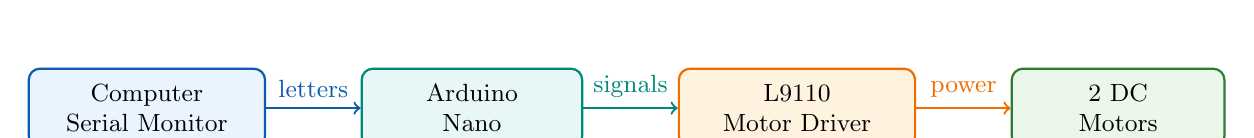
\begin{tikzpicture}[node distance=1.2cm, every node/.style={font=\small, align=center}]
  \node[draw=LabBlue, fill=LabLightBlue, rounded corners, thick, minimum width=3.0cm, minimum height=1.0cm] (pc) {Computer\\Serial Monitor};
  \node[draw=LabTeal, fill=LabLightTeal, rounded corners, thick, right=of pc, minimum width=2.8cm, minimum height=1.0cm] (arduino) {Arduino\\Nano};
  \node[draw=LabOrange, fill=LabLightOrange, rounded corners, thick, right=of arduino, minimum width=3.0cm, minimum height=1.0cm] (driver) {L9110\\Motor Driver};
  \node[draw=LabGreen, fill=LabLightGreen, rounded corners, thick, right=of driver, minimum width=2.7cm, minimum height=1.0cm] (motors) {2 DC\\Motors};
  \draw[->, thick, LabBlue] (pc) -- node[above]{letters} (arduino);
  \draw[->, thick, LabTeal] (arduino) -- node[above]{signals} (driver);
  \draw[->, thick, LabOrange] (driver) -- node[above]{power} (motors);
\end{tikzpicture}
\end{center}

\section*{\textcolor{LabBlue}{3. Materials}}

\begin{tabularx}{\linewidth}{>{\bfseries}p{0.32\linewidth}X}
Arduino Nano & Receives commands from the computer and sends signals to the motor driver.\\
L9110 2-channel motor driver & Controls the direction and speed of two DC motors.\\
Two DC motors & Move the robot.\\
External motor battery or power supply & Powers the motors through the L9110 driver.\\
USB cable & Uploads code and opens the Serial Monitor.\\
Jumper wires & Connect the Arduino, driver, and power supply.\\
\end{tabularx}

\colourbox{LabRed}{LabLightOrange}{
  \textbf{\textcolor{LabRed}{Safety and Care}}\\
  Do not power the motors only from the Arduino Nano 5V pin or USB. Use an
  external motor battery or power supply. Always connect Arduino GND and motor
  battery GND together.
}

\section*{\textcolor{LabBlue}{4. Wiring Checklist}}

Connect the L9110 input pins to the Arduino Nano:

\begin{center}
  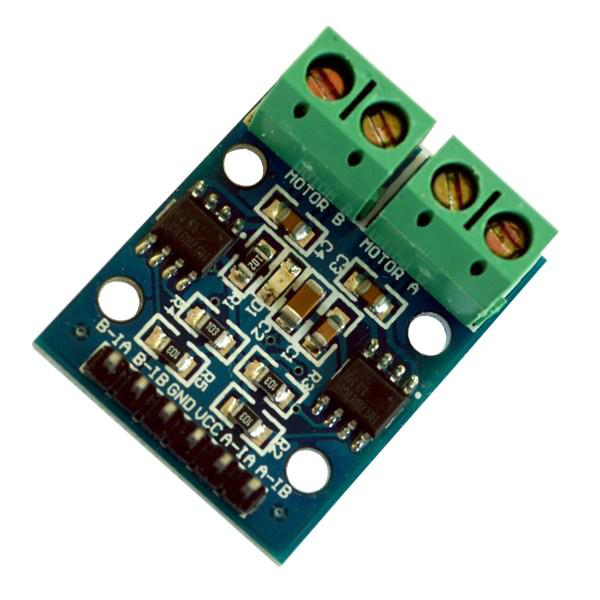
\includegraphics[width=0.40\linewidth]{assets/l9110_driver.png}\\[-0.2em]
  {\small \textbf{L9110 2-channel motor driver.} The six-pin header is labelled
  B-IA, B-IB, GND, VCC, A-IA, and A-IB. The green screw terminals connect to
  Motor A and Motor B.}
\end{center}

\begin{center}
\rowcolors{2}{LabLightBlue}{white}
\begin{tabular}{>{\bfseries}c c}
\rowcolor{LabBlue}
\textcolor{white}{L9110 Pin} & \textcolor{white}{Arduino Nano Pin}\\
A-IA & D3\\
A-IB & D5\\
B-IA & D6\\
B-IB & D9\\
GND & Arduino GND and battery GND\\
VCC & External motor power, usually 2.5V to 12V\\
\end{tabular}
\end{center}

\colourbox{LabPurple}{LabLightPurple}{
  \textbf{\textcolor{LabPurple}{Before You Upload}}\\
  Ask your teacher to check your wiring before turning on motor power. A wiring
  mistake can make the robot behave strangely or stop the upload from working.
}

\section*{\textcolor{LabBlue}{5. Arduino IDE Setup}}

\begin{enumerate}
  \item Open the Arduino IDE.
  \item Open the robot code file.
  \item Select \textbf{Tools \(\rightarrow\) Board \(\rightarrow\) Arduino AVR Boards \(\rightarrow\) Arduino Nano}.
  \item Select \textbf{Tools \(\rightarrow\) Processor \(\rightarrow\) ATmega168}.
  \item Select the correct \textbf{Tools \(\rightarrow\) Port}.
  \item Upload the code.
  \item Open \textbf{Tools \(\rightarrow\) Serial Monitor}.
  \item Set the baud rate to \textbf{9600}.
\end{enumerate}

\colourbox{LabOrange}{LabLightOrange}{
  \textbf{\textcolor{LabOrange}{Nano Upload Tip}}\\
  This lab uses an Arduino Nano with an \textbf{ATmega168} processor. If uploading
  fails, check that \textbf{Tools \(\rightarrow\) Processor \(\rightarrow\) ATmega168}
  is selected.
}

\section*{\textcolor{LabBlue}{6. Serial Monitor Commands}}

Type one command and press Send.

\begin{center}
\rowcolors{2}{LabLightTeal}{white}
\begin{tabular}{>{\centering\arraybackslash\bfseries}p{0.15\linewidth} p{0.55\linewidth}}
\rowcolor{LabTeal}
\textcolor{white}{Command} & \textcolor{white}{Robot Action}\\
F & Move forward\\
B & Move backward\\
L & Turn left\\
R & Turn right\\
S & Stop\\
+ & Increase speed\\
- & Decrease speed\\
? & Show the help menu\\
\end{tabular}
\end{center}

\section*{\textcolor{LabBlue}{7. Experiment Procedure}}

\subsection*{\textcolor{LabTeal}{Part A: First Contact}}

\begin{enumerate}
  \item Open the Serial Monitor.
  \item Send \texttt{?}.
  \item Write down what appears on the screen.
\end{enumerate}

\colourbox{LabGreen}{LabLightGreen}{
  \textbf{Observation:} What did the Arduino print after you sent \texttt{?}?\\[1.5em]
  \hrulefill
}

\subsection*{\textcolor{LabTeal}{Part B: Test Each Movement}}

Send each command and record what the robot does.

\begin{center}
\rowcolors{2}{LabLightBlue}{white}
\begin{tabularx}{\linewidth}{>{\bfseries}c X X}
\rowcolor{LabBlue}
\textcolor{white}{Command} & \textcolor{white}{Expected Movement} & \textcolor{white}{What Actually Happened?}\\
F & Forward & \\
B & Backward & \\
L & Turn left & \\
R & Turn right & \\
S & Stop & \\
\end{tabularx}
\end{center}

\subsection*{\textcolor{LabTeal}{Part C: Test Speed}}

\begin{enumerate}
  \item Send \texttt{F}.
  \item Send \texttt{+} two times.
  \item Send \texttt{-} two times.
  \item Send \texttt{S}.
\end{enumerate}

\colourbox{LabGreen}{LabLightGreen}{
  \textbf{Observation:} How did the robot change when the speed changed?\\[1.5em]
  \hrulefill
}

\subsection*{\textcolor{LabTeal}{Part D: Mini Challenge}}

Write a sequence of commands to make your robot:

\begin{itemize}
  \item move forward,
  \item turn around,
  \item come back,
  \item stop.
\end{itemize}

\colourbox{LabPurple}{LabLightPurple}{
  \textbf{Your command sequence:}\\[1.5em]
  \hrulefill\\[1.5em]
  \hrulefill
}

\section*{\textcolor{LabBlue}{8. What Is Happening in the Code?}}

\begin{tabularx}{\linewidth}{>{\bfseries}p{0.24\linewidth}X}
\texttt{setup()} & Runs once. It sets the motor pins as outputs, starts Serial communication, and prints the help menu.\\
\texttt{loop()} & Runs again and again. It checks if a new Serial Monitor command arrived.\\
\texttt{Serial.read()} & Reads one character from the Serial Monitor.\\
\texttt{forward()} & Sends PWM to the correct L9110 input pins so both motors spin forward.\\
\texttt{backward()} & Reverses which input pins receive PWM, so both motors spin backward.\\
\texttt{stopMotors()} & Sets all L9110 input pins LOW, stopping both motors.\\
\texttt{analogWrite()} & Sends a PWM value from 0 to 255 to control motor speed.\\
\end{tabularx}

\colourbox{LabOrange}{LabLightOrange}{
  \textbf{\textcolor{LabOrange}{Why does the robot pause before moving?}}\\
  The code stops the motors for 400 ms before each new movement. This gives the
  motor driver and motors time to settle before changing direction.
}

\section*{\textcolor{LabBlue}{9. Expected Problems and Fixes}}

\begin{center}
\rowcolors{2}{LabLightOrange}{white}
\begin{tabularx}{\linewidth}{>{\bfseries}p{0.26\linewidth}X X}
\rowcolor{LabOrange}
\textcolor{white}{Problem} & \textcolor{white}{Possible Cause} & \textcolor{white}{What To Try}\\
Nothing moves & Motor power is missing, or GND is not shared & Check L9110 VCC, battery, Arduino GND, and battery GND.\\
Serial Monitor shows nothing & Wrong baud rate or wrong port & Set Serial Monitor to 9600 and check Tools \(\rightarrow\) Port.\\
Upload fails & Wrong Nano processor setting & Select Tools \(\rightarrow\) Processor \(\rightarrow\) ATmega168.\\
Robot goes backward when you send F & Motor wires are reversed & Swap the two wires on each motor.\\
Left and right are reversed & Motor A and Motor B are swapped, or one motor is wired backwards & Swap motor sides or reverse one motor's wires.\\
One motor moves but the other does not & Loose wire or wrong pin & Check D3, D5, D6, D9 and motor screw terminals.\\
Robot only changes direction after Stop & Motor driver needs a pause before reversing & Make sure the code includes the 400 ms pause before movement.\\
Robot resets when motors start & Motor current is too high for the supply & Use a stronger battery or reduce speed.\\
\end{tabularx}
\end{center}

\section*{\textcolor{LabBlue}{10. Reflection Questions}}

Answer in full sentences.

\begin{enumerate}
  \item Why do we use an L9110 motor driver instead of connecting the motors directly to the Arduino?
  \vspace{2em}

  \item What does the Arduino receive when you type \texttt{F} in the Serial Monitor?
  \vspace{2em}

  \item What is PWM? Why is a value like 200 different from 255?
  \vspace{2em}

  \item Why should the Arduino GND and motor battery GND be connected together?
  \vspace{2em}

  \item If your robot moves in the wrong direction, what evidence would help you decide what to change?
  \vspace{2em}

  \item What is one improvement you would make to this robot if you had more time?
  \vspace{2em}
\end{enumerate}

\section*{\textcolor{LabBlue}{11. Exit Ticket}}

\colourbox{LabBlue}{LabLightBlue}{
  \textbf{In one or two sentences:} What did you learn today about how computers control motion?\\[3em]
  \hrulefill\\[1.5em]
  \hrulefill
}

\section*{\textcolor{LabBlue}{12. Teacher Check}}

\colourbox{LabTeal}{LabLightTeal}{
  \textbf{\textcolor{LabTeal}{Teacher Checklist}}\\[0.4em]
  \begin{tabularx}{\linewidth}{>{\bfseries}p{0.58\linewidth}X}
    \checkboxitem{Wiring checked} & Notes: \hrulefill\\[1.0em]
    \checkboxitem{Code uploaded} & Notes: \hrulefill\\[1.0em]
    \checkboxitem{Robot responds to Serial Monitor} & Notes: \hrulefill\\[1.0em]
    \checkboxitem{Students completed observations} & Notes: \hrulefill\\[1.0em]
    \checkboxitem{Students answered reflection questions} & Notes: \hrulefill\\
  \end{tabularx}
}

\end{document}
